\documentclass[12pt,a4paper]{article}
\usepackage[utf8]{inputenc}
\usepackage[spanish]{babel}
\usepackage{amsmath}
\usepackage{amsfonts}
\usepackage{amssymb}
\usepackage{graphicx}
\usepackage{titlesec}
\usepackage{titling}
\usepackage[left=3cm,right=2cm,top=2cm,bottom=2cm]{geometry}
\date{\small{\today}}
\usepackage{fancyhdr}
\usepackage{afterpage}
\usepackage{cancel}
\usepackage[usenames,dvipsnames,svgnames,table]{xcolor}
\definecolor{gris}{RGB}{220,220,220}

\titleformat{\section}{\Large\bfseries}{}{0em}{}[\titlerule]
\titleformat{\subsection}{\large\bfseries}{}{0em}{}[]

\begin{document}



%caratula
  \begin{center}


    
\includegraphics[scale=0.15]{ib}
    \vspace{1cm}
    \vspace{1cm}
    \\
    \Huge{INSTITUTO BALSEIRO}
    \vspace{2cm}\\
    \huge{\textbf{Ingreso 2019}}\\
    \vspace{1cm}
    \LARGE{Resumen de fórmulas}\\
    \vspace{1cm}
    \large
    \begin{flushleft}

      $-$Autor:\\
      \begin{itemize}

        \item[$+$] Nadia A. Pizarro.
        \item[$+$] Matías D. Roqueta.

      \end{itemize}

    \end{flushleft}
    \vspace{0,5cm}

    \today
    \thispagestyle{empty}
  \end{center}



\lhead{}
\rhead{Ingreso 2019} % Logo
\chead{Sección: \thesection.\thesubsection}
%\ Pie
\lfoot{Nadia A. Pizarro. \\ Matías D. Roqueta}
\cfoot{Instituto Balseiro} % quitar número de página del centro
\rfoot{\thepage} % número de página a la derecha
\renewcommand{\headrulewidth}{0.4pt} % grosor de la línea de la cabecera
\renewcommand{\footrulewidth}{0.4pt} % grosor de la línea del pie
\pagestyle{fancy}

%indice

\newpage

\tableofcontents
\newpage

%desarrollo
\begin{quote}
\begin{center}

\abstractname{\textit{ : En el siguiente artículo hare un resumen de las fórmulas y conceptos que repasaré una vez terminado de estudiar todos los temas, no es un resumen de todo lo que sé ni de todo lo que estudié, espero que también le sirva a alguien más.}}

\end{center}
\end{quote}

\section{Análisis Matemático}

\textbf{Derivadas:}
\begin{itemize}
  \item $ \sen(x) \rightarrow \cos(x)$
  \item $ \cos(x) \rightarrow -\sen(x)$
  \item $ \ln(x) \rightarrow \dfrac{1}{x}$
  \item $ \tg(x) \rightarrow \dfrac{1}{\cos^2(x)}$
  \item $ \cotg(x) \rightarrow \dfrac{-1}{\sen^2(x)}$
  \item $ \arcsen(x) \rightarrow \dfrac{1}{\sqrt{1-x^2}}$
  \item $ \arccos(x) \rightarrow \dfrac{-1}{\sqrt{1-x^2}}$
  \item $ \arctg(x) \rightarrow \dfrac{1}{1+x^2}$
\end{itemize}

\textbf{Diferencial:} \\
El valor exacto de un incremento esta dado por $\Delta z = F(x+\Delta x; y +\Delta y )  F(x;y)$ Mientras que podemos obtener un valor aproximado con el diferencial: $dz= \dfrac{\partial F}{\partial x}\cdot dx +\dfrac{\partial F}{\partial y}\cdot dy $. Podemos decir que $\Delta x = dx$ y $\Delta y = dy$ pero $\Delta z \neq dz$, aunque para valores muy pequeños se aproximan.  \\

  \textbf{Dominio de una función:} Debemos restringir el dominio y si se puede graficarlo con las siguientes reglas:
  \begin{itemize}
     \item En los radicales el argumento tiene que ser $ \geq 0$.
     \item El denominador de una fracción debe ser $\neq 0$.
     \item El argumento del logaritmo debe ser $> 0$.

  \end{itemize}

  \textbf{Derivada direccional:}\\
  Se define la derivada direccional de F con respecto al vector $\vec{v}$ como :
  $$\dfrac{\partial F(x;y)}{\partial \vec{v}} = \dfrac{\partial F}{\partial x} \cdot \cos(\alpha)+ \dfrac{\partial F }{\partial y} \cdot \sen(\alpha) $$
  Si el vector $\vec{v}$ esta normalizado se puede escribir como:
  $$\dfrac{\partial F(x;y)}{\partial \vec{v}}=\nabla F \cdot \vec{v}_{normalizado}$$\\
  De no estar normalizado debemos hacerlo como:
  $$\vec{v}_{normalizado}= \dfrac{\vec{v}}{|\vec{v}|}$$
  \\
  La \textcolor{red}{derivada direccional máxima} es cuando la dirección es la del gradiente en ese punto, mientras que la \textcolor{blue}{derivada direccional mínima} es la misma dirección del gradiente pero de sentido contrario, esto se logra con la multiplicación punto del vector gradiente por el escalar (-1). La \textcolor{green}{derivada direccional nula} será usando un vector tal que sea perpendicular al vector en la derivada direccional máxima.\\

  \textbf{Regla de la cadena mutlivariable:}
  Se divide en los siguientes casos:
  \begin{itemize}
    \item \textit{caso 1:} La funcion $F$ tiene como variable de entrada a $t/t \in \Re$, teniendo a dos variables intermedias $x(t) \wedge y(t)/ x \wedge y \in \Re $ y teniendo como salida una variable llamada $z/z\in \Re$, se define la derivada de $z$ con respecto a $t$ como:
    $$\dfrac{dz}{dt}=\dfrac{\partial z}{\partial x}\cdot \dfrac{d x}{dt}+\dfrac{\partial z}{\partial y}\cdot \dfrac{dy}{dt}$$
    \item \textit{caso 1 particular:}La funcion $F$ tiene como variable de entrada a $x/x \in \Re$, teniendo a dos variables intermedias $x(t) \wedge y(t)/ x \wedge y \in \Re $ y teniendo como salida una variable llamada $z/z\in \Re$, se define la derivada de $z$ con respecto a $x$ como:
    $$\dfrac{dz}{dx}=\dfrac{\partial z}{\partial x}\cdot \cancelto{1}{\dfrac{d x}{dx}}+\dfrac{\partial z}{\partial y}\cdot \dfrac{dy}{dx}$$
    \item \textit{caso 2:} La funcion $F$ tiene como variable de entradas a $u\wedge v/u\wedge v \in \Re$, teniendo a dos variables intermedias$x(t)\wedge y(t)/ x\wedge y \in \Re$ y como salida una sola variable llamada $z(x,y)/z \in \Re$, se define la derivada parcial de $z$ con respecto a $u$ como:
    $$ \dfrac{\partial z}{\partial u} =\dfrac{\partial z}{\partial x} \cdot \dfrac{\partial x}{\partial u}+\dfrac{\partial z}{\partial y}\cdot \dfrac{\partial y}{\partial u}$$
    Y se define la derivada parcial de $z$ con respecto a $v$ como:
   $$ \dfrac{\partial z}{\partial v} =\dfrac{\partial z}{\partial x} \cdot \dfrac{\partial x}{\partial v}+\dfrac{\partial z}{\partial y}\cdot \dfrac{\partial y}{\partial v}$$

    \item \textit{caso 2, 1er caso particular:}La funcion $F$ tiene como variable de entradas a $u\wedge v/u \wedge v \in \Re$, teniendo a dos variables intermedias$u(u,v)\wedge y(u,v)/ u\wedge y \in \Re$ y como salida una sola variable llamada $z(x,y)/z \in \Re$, se define la derivada parcial de $z$ con respecto a $u$ como:
    $$ \dfrac{\partial z}{\partial u} =\dfrac{\partial z}{\partial u} \cdot \cancelto{1}{\dfrac{\partial u}{\partial u}}+\dfrac{\partial z}{\partial y}\cdot \dfrac{\partial y}{\partial u}$$
    Y se define la derivada parcial de $z$ con respecto a $v$ como:
   $$ \dfrac{\partial z}{\partial v} =\dfrac{\partial z}{\partial u} \cdot \cancelto{0}{\dfrac{\partial u}{\partial v}}+\dfrac{\partial z}{\partial y}\cdot \dfrac{\partial y}{\partial v}$$
   La $\dfrac{\partial u}{\partial v}=0 $ porque $u$ y $v$ son variables independientes y la derivada de una constante es 0.\\
   \item \textit{caso 2, 2do caso particular}La funcion $F$ tiene como variable de entradas a $x\wedge y/x \wedge y \in \Re$, teniendo a dos variables intermedias$x\wedge y\wedge z/ x\wedge y \wedge z \in \Re$ y como salida una sola variable llamada $w(x,y,z)/w \in \Re$, se define la derivada parcial de $w$ con respecto a $x$ como:
   $$ \dfrac{\partial w}{\partial x} =\dfrac{\partial w}{\partial x} \cdot \cancelto{1}{\dfrac{\partial x}{\partial x}}+\dfrac{\partial w}{\partial y}\cdot \cancelto{0}{\dfrac{\partial y}{\partial x}} +\dfrac{\partial w}{\partial z}\cdot \dfrac{\partial z}{\partial x}$$
   Y se define la derivada parcial de $w$ con respecto a $y$ como:
  $$ \dfrac{\partial w}{\partial y} =\dfrac{\partial w}{\partial x} \cdot \cancelto{0}{\dfrac{\partial x}{\partial y}}+\dfrac{\partial w}{\partial y}\cdot \cancelto{1}{\dfrac{\partial y}{\partial y}}+\dfrac{\partial w}{\partial z}\cdot \dfrac{\partial z}{\partial y}$$
  La $\dfrac{\partial y}{\partial x}= \dfrac{\partial x}{\partial y}=0 $ porque $x$ y $y$ son variables independientes y la derivada de una constante es 0.\\
\end{itemize}

\textbf{Extremos relativos:}\\
Condición \textit{necesaria} para que haya un extremo:
$$\dfrac{\partial z}{\partial x}=0$$
$$\dfrac{\partial z}{\partial y}= 0$$
Esto nos dará un sistema de ecuaciones y los valores que cumplan con la ecuación serán puntos críticos.\\
Condición \textit{suficiente} El hessiano en ese punto nos dirá mas información sobre ese punto. Se define el Hessiano como:\\
$$
Hess =
\begin{bmatrix}
\dfrac{\partial ^2 z}{\partial x^2 } &  \dfrac{\partial ^2 z}{\partial y \partial x} \\
\dfrac{\partial ^2 z}{\partial x \partial y} & \dfrac{\partial ^2 z}{\partial y^2}
\end{bmatrix}
$$
\\
Se calcula el determinante de la matriz, evaluado en el punto crítico entonces:Ay 
\begin{itemize}
\item Si $det(Hess) > 0$ hay un extremo.  En ese caso si $Hes_{11} = \dfrac{\partial ^2 z}{\partial x^2} \textcolor{violet}{>} 0$ hay un \textcolor{violet}{mínimo} relativo.  En cambio si $Hess_{11} =  \dfrac{\partial ^2 z}{\partial y^2} \textcolor{green}{<} 0$ hay un \textcolor{green}{máximo} relativo. \textcolor{red}{Atención!!} Los signos no son intuitivos, estan intercalados.

\item Si $det(Hess) = 0$ el criterio no decide y debemos buscar otra forma de analizar el punto crítico.

\item Si $det(Hess) < 0$ entonces hay un punto silla y por lo tanto no es extremo.
\end{itemize}


\textbf{Divergencia:} cambio de densidad en el movimiento de una partícula. Se define con la eq:
 $ \nabla  \cdot \vec{V} = Div \vec{V}$. En la figura \ref{fig:divergencia} se puede observar que quiere decir el escalar que nos dá de resultado.\\

 \begin{figure}[htbp]
   \begin{center}
       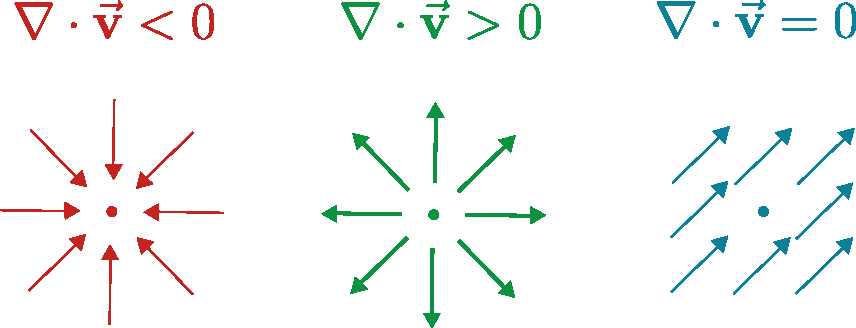
\includegraphics[scale=0.8]{divergencia.pdf}
     \caption{Interpretación de la divergencia}
     \label{fig:divergencia}
   \end{center}
 \end{figure}



 \textbf{Rotacional:} Si una función que toma valores de vectores tridimensionales  $\vec{\textbf{v}}(x,y,z)$ tiene como funciones componentes a $\textcolor{blue}{v_1}(x,y,z)$, $\textcolor{red}{v_2}(x,y,z)$ y $\textcolor{green}{v_3}(x,y,z)$, entonces el rotacional se calcula de la siguiente manera:
$$\nabla \times \vec{\textbf{v}}  = \left( \dfrac{\partial \textcolor{green}{v_3}}{\partial y}- \dfrac{\partial \textcolor{red}{v_2}}{\partial z} \right)\hat{\textbf{i}} + \left( \dfrac{\partial \textcolor{blue}{v_1}}{\partial z}-  \dfrac{\partial \textcolor{green}{v_3}}{\partial x} \right)\hat{\textbf{j}} + \left( \dfrac{\partial \textcolor{red}{v_2}}{\partial x}- \dfrac{\partial \textcolor{blue}{v_1}}{\partial y} \right)\hat{\textbf{k}} $$
\\
Tambien se puede calcular como:
$$\nabla\times \vec{\textbf{v}}=\left|
\begin{matrix} \hat i & \hat j & \hat k  \\ & & \\
\cfrac{\partial}{\partial x} & \cfrac{\partial}{\partial y} & \cfrac{\partial}{\partial z}
\\ & & \\ \textcolor{blue}{v_1} & \textcolor{red}{v_2} & \textcolor{green}{v_3}  \end{matrix}\right|$$
\\


\textbf{Teorema fundamental del cálculo:} Dada unafunción $f$ integrable sobre el intervalo $ [a,b]$, definimos $F$ sobre $[a,b]$ por $F(x) = {\int_{a}^x f(t)dt}$. Si $f$ es continua en $c \notin (a,b)$, entonces $F$ es derivable en $c$ y $F'(c) = f(c)$.\\

\textbf{Plano tangente o aproximación lineal:} La ecuación del plano tangente de la gráfica de una función de dos variables f(x,y) en un punto particular $(x_0, y_0)$ se ve así:
$$T(x, y) = f(x_0, y_0) + {f_{\textcolor{blue}{x}}(x_0, y_0)}(\textcolor{blue}{x}-x_0) + {f_{\textcolor{red}{y}}(x_0, y_0)}(\textcolor{red}{y}-y_0) $$

\textbf{Aproximación cuadrática:} La ecuación de una función que se aproxima cuadrátcamente a una función de dos variables f(x,y) en un punto particular $(x_0, y_0)$ se ve así:
$$ C(x, y) = f(x_0, y_0) + {f_{\textcolor{blue}{x}}(x_0, y_0)}(\textcolor{blue}{x}-x_0) + {f_{\textcolor{red}{y}}(x_0, y_0)}(\textcolor{red}{y}-y_0)+\frac{1}{2} \cdot f_{\textcolor{blue}{xx}}(x_0, y_0)(\textcolor{blue}{x}-x_0)^2+ \cdots $$
  $$\cdots + f_{\textcolor{red}{y}\textcolor{blue}{x}}(x_0, y_0)(\textcolor{blue}{x}-x_0)(\textcolor{red}{y}-y_0)+ \frac{1}{2} \cdot {f_{\textcolor{red}{yy}}(x_0, y_0)}(\textcolor{red}{y}-y_0)^2 $$

\newpage

\section{Mecánica Clásica}
\textbf{Ley de Newton:} La sumatoria de fuerzas sobre un cuerpo equivale a la variación de su momento lineal respecto al tiempo.\\
$$\sum{\vec{F}} = \dfrac{d\vec{p}}{dt} = m \, \dfrac{d\vec{v}}{dt} + \dfrac{dm}{dt} \, \vec{v}$$.
Solo en el caso de masa invariante en el tiempo la expresión se reduce a $\sum {\vec{F}} = m \, \vec{a}$\\

Análogamente, la sumatoria de torque sobre un cuerpo equivale a la variación temporal de su momento angular, en caso de momento de momento de inercia invariante en el tiempo reducida a $\sum {\vec{T}} = I \, \vec{\alpha}$\\

\textbf{Momento de Inercia:} Así como la masa cuantifica la dificultad de alterar el estado de movimiento de un cuerpo, el momento de inercia cuantifica su resistencia a cambiar su estado de movimiento rotacional \emph{respecto a un determinado eje}. La fórmula general para encontrarlo para un cuerpo cualquiera con densidad volumétrica $\rho(\vec r)$ es.
$$I_0 = \int_{V}r^2 \, \rho(\vec{r})\, dV$$
Los momentos de inercia baricéntricos de los rígidos de masa uniforme mas comunes son conocidos.\\

\textbf{Torque o Momento de Fuerza: } Es el resultado de un \textcolor{blue}{par de fuerzas} paralelas, de igual módulo, y sentido contrario.
Siendo la distancia-vector entre los puntos de aplicación de las dos fuerzas $\vec{r}$, se cumple.
$$\vec{T}=\vec{r}\times\vec{F}$$
En muchas ocasiones, una de estas fuerzas es la llamada \textcolor{blue}{fuerza de vínculo}, la fuerza que ejerce un eje de rotación fijo sobre un cuerpo para impedir su desplazamiento.\\

\begin{figure}[htbp]
	\begin{center}
		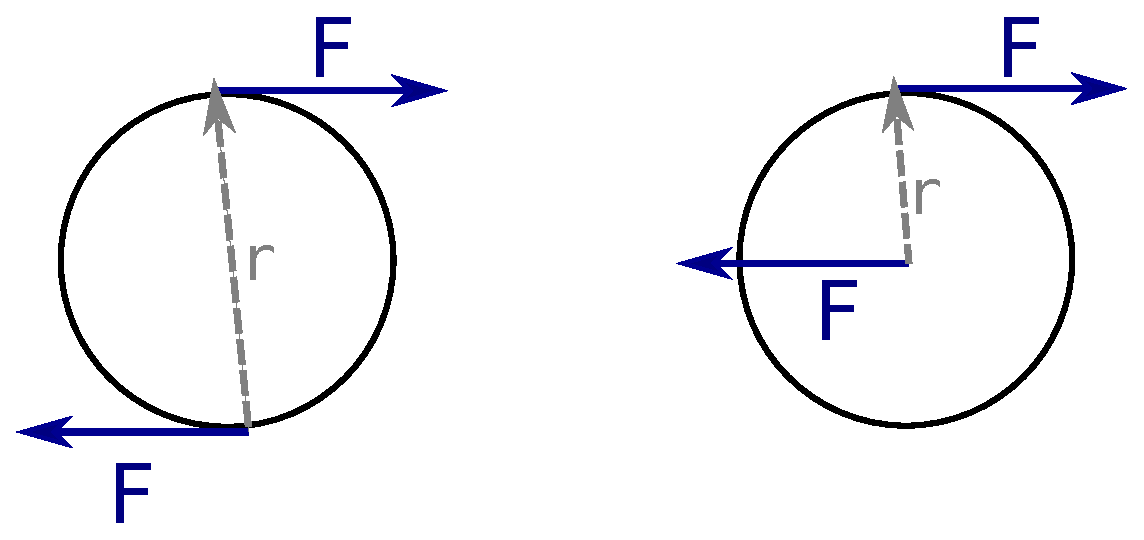
\includegraphics[width=0.6\textwidth]{torque.eps}
		\caption{Dos posibles ejemplos de torque. A la derecha, un par de fuerzas independientes iguales y contrarias actuando sobre un rígido. A la derecha una fuerza externa actuando sobre un rígido fijo en un eje y la fuerza de vínculo.}
		\label{fig:torque}
	\end{center}
\end{figure}

\textbf{Teorema de Steiner:} Si se conoce el momento de inercia de un cuerpo rígido respecto a su eje baricéntrico $I_0$, el teorema de Steiner establece su momento de inercia respecto a cualquier otro eje paralelo a este a una distancia $r'$.
$$I = I_0 + m \, r'^2$$

\subsection{Leyes de Conservación} 
En todo sistema mecánico considerando un intervalo temporal arbitrario $\Delta t$ se cumplen las siguientes leyes de conservación.\\

\begin{itemize}
	\item \textbf{Ley de Conservación de la Energía Mecánica}. La sumatoria de trabajo ejercido por \textcolor{red}{fuerzas no conservativas} es igual a la variación de energía mecánica del sistema. $$\sum{W_{F_{NC}}} = \Delta E_M$$.
	\item \textbf{Ley de Conservación del Momento Lineal}. La sumatoria de impulso lineal ejercido sobre el sistema por \textcolor{blue}{fuerzas externas} es igual a la variación del momento lineal del sistema. $$\sum{\vec{J}_{F_{ext}}} = \Delta \vec{p}$$.
	\item \textbf{Ley de Conservación del Momento Angular}.La sumatoria de impulso angular ejercido sobre el sistema por torque producto de \textcolor{blue}{fuerzas externas} es igual a la variación del momento angular del sistema.
	$$\sum{\vec{J}_{T_{ext}}} = \Delta \vec{L}$$.
\end{itemize}

\textbf{Fuerzas Internas:} \textcolor{blue}{Fuerzas internas} son todas aquellas en las que ambas partes del par acción-reacción están aplicadas sobre elementos del sistema.\\

\textbf{Fuerzas Conservativas:} \textcolor{red}{Fuerza conservativa} es toda fuerza asociada a un campo conservativo, por ende puede asociar una función Potencial. \textit{<insertar referencia a capítulo de análisis matemático>}\\

\textbf{Trabajo:} Integral de una fuerza aplicada sobre una trayectoria. $\displaystyle W=\int_{\vec{x}_1}^{\vec{x}_2}\vec{F}(\vec{x})\cdot d\vec{x}$

\textbf{Impulso Lineal:} Integral de la fuerza en el tiempo. $\displaystyle \vec{J}=\int_{t_1}^{t_2}\vec{F}(t)\, dt$

\textbf{Impulso Angular:} Integral de un torque en el tiempo. $\displaystyle  \vec{J}_T=\int_{t_1}^{t_2}\vec{T}(t)\, dt$ \\

\textbf{Momento Lineal} Magnitud \textcolor{red}{vectorial} e \textcolor{blue}{instantánea} que representa la cantidad de movimiento rectilíneo de un cuerpo. $\displaystyle \vec{p}=m \, \vec{v}$ \\

\textbf{Momento Angular} Magnitud \textcolor{red}{vectorial} e \textcolor{blue}{instantánea} que representa la cantidad de movimiento angular de un cuerpo. La dirección del vector representa la dirección normal al plano donde se desarrolla la rotación.

Existen dos formas de tener momento angular, intrínseco y orbital. El momento angular total es la suma de los dos.

\begin{itemize}
	\item \textbf{$\vec{L}$ intrínseco:} o \textit{spin}, momento angular de un cuerpo rígido por tener velocidad angular instantánea respecto a su propio eje. $$\vec{L}_{spin} = I \, \vec{\omega}$$
	

	\item \textbf{$\vec{L}$ orbital:} Momento angular de un cuerpo por instantáneamente orbitar con un determinado momento lineal, a un radio vector $\vec{r}$ de un determinado eje. $$\vec{L}_{orbit} = \vec{r} \times \vec{p}$$
\end{itemize}

El momento angular total de un cuerpo o sistema resulta la suma de ambas formas de momento angular, siempre manteniendo consistente el eje de referencia: $\displaystyle \vec{L}=\vec{L}_{spin}+\vec{L}_{orbit}$


<INSERTAR COSAS DE ENERGÍA MECÁNICA> \\

\newpage
\subsection{Movimiento Oscilatorio Armónico Simple} 
La ecuación que define un movimiento oscilatorio es una ecuación diferencial ordinaria de segundo orden de la siguiente forma:
$$\dfrac{d^2y(t)}{dt^2} + A y(t) = 0$$

Los sistemas oscilatorios armónicos simples son aquellos en los que ejerce trabajo únicamente una fuerza conservativa de acción restitutiva, actuando hacia una posición de equilibrio inversamente proporcional a la posición.\\

La solución es conocida, y es de la forma 
$$y(t) = A \sin\left(\omega_0t+\phi\right)$$
Resolviendo la ecuación se puede encuentra la frecuencia natural del sistema oscilatorio $\omega_0$, y de las condiciones iniciales saldrán la amplitud y fase, $A$ y $\phi$. \\

\textbf{Energía del Sistema Oscilatorio:} Por teorema de conservación de la energía, se encuentra que la \textcolor{green}{energía mecánica} total del oscilador permanece constante. Se manifiesta únicamente un intercambio entre \textcolor{blue}{energía potencial} y \textcolor{red}{energía cinética}. Esta propiedad facilita cualquier cálculo de tipo energético.   

\begin{figure}[htbp]
	\begin{center}
		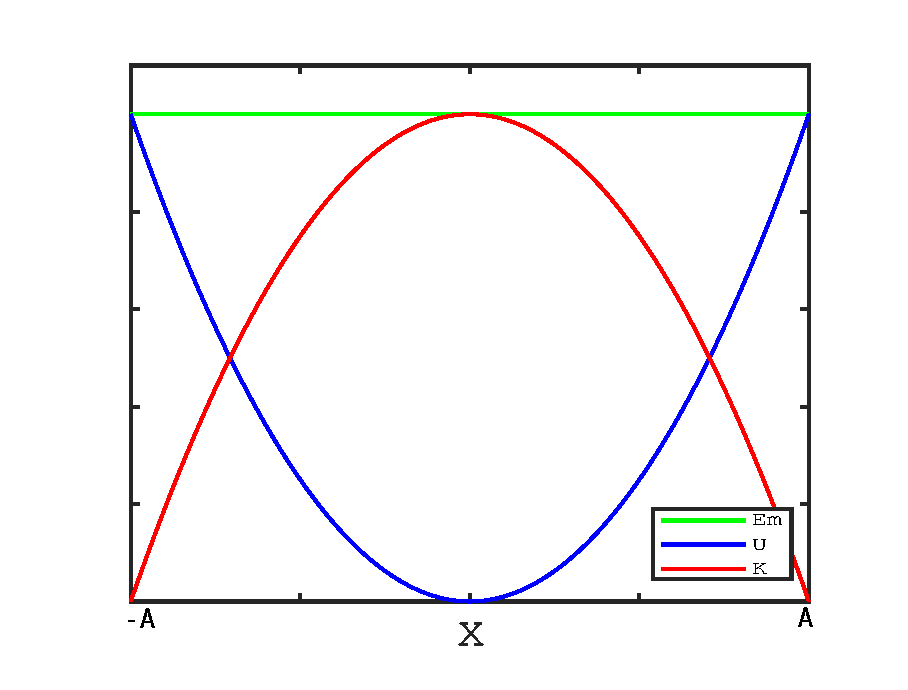
\includegraphics[scale=0.75]{energOscil.eps}
		\caption{Representación gráfica de energía en un oscilador mecánico}
		\label{fig:energOscil}
	\end{center}
\end{figure}


\end{document}

